% % % % % % % % % % % % % % % % % % % % % % % % % % % % % % % % % % % % % % % % %
% INTRO
% % % % % % % % % % % % % % % % % % % % % % % % % % % % % % % % % % % % % % % % %
\section{Time box 6}
\listoftodos
\subsection{Time box planning}

\begin{figure}[H]
	\begin{centering}
		\missingfigure{Updated timebox figure}
		%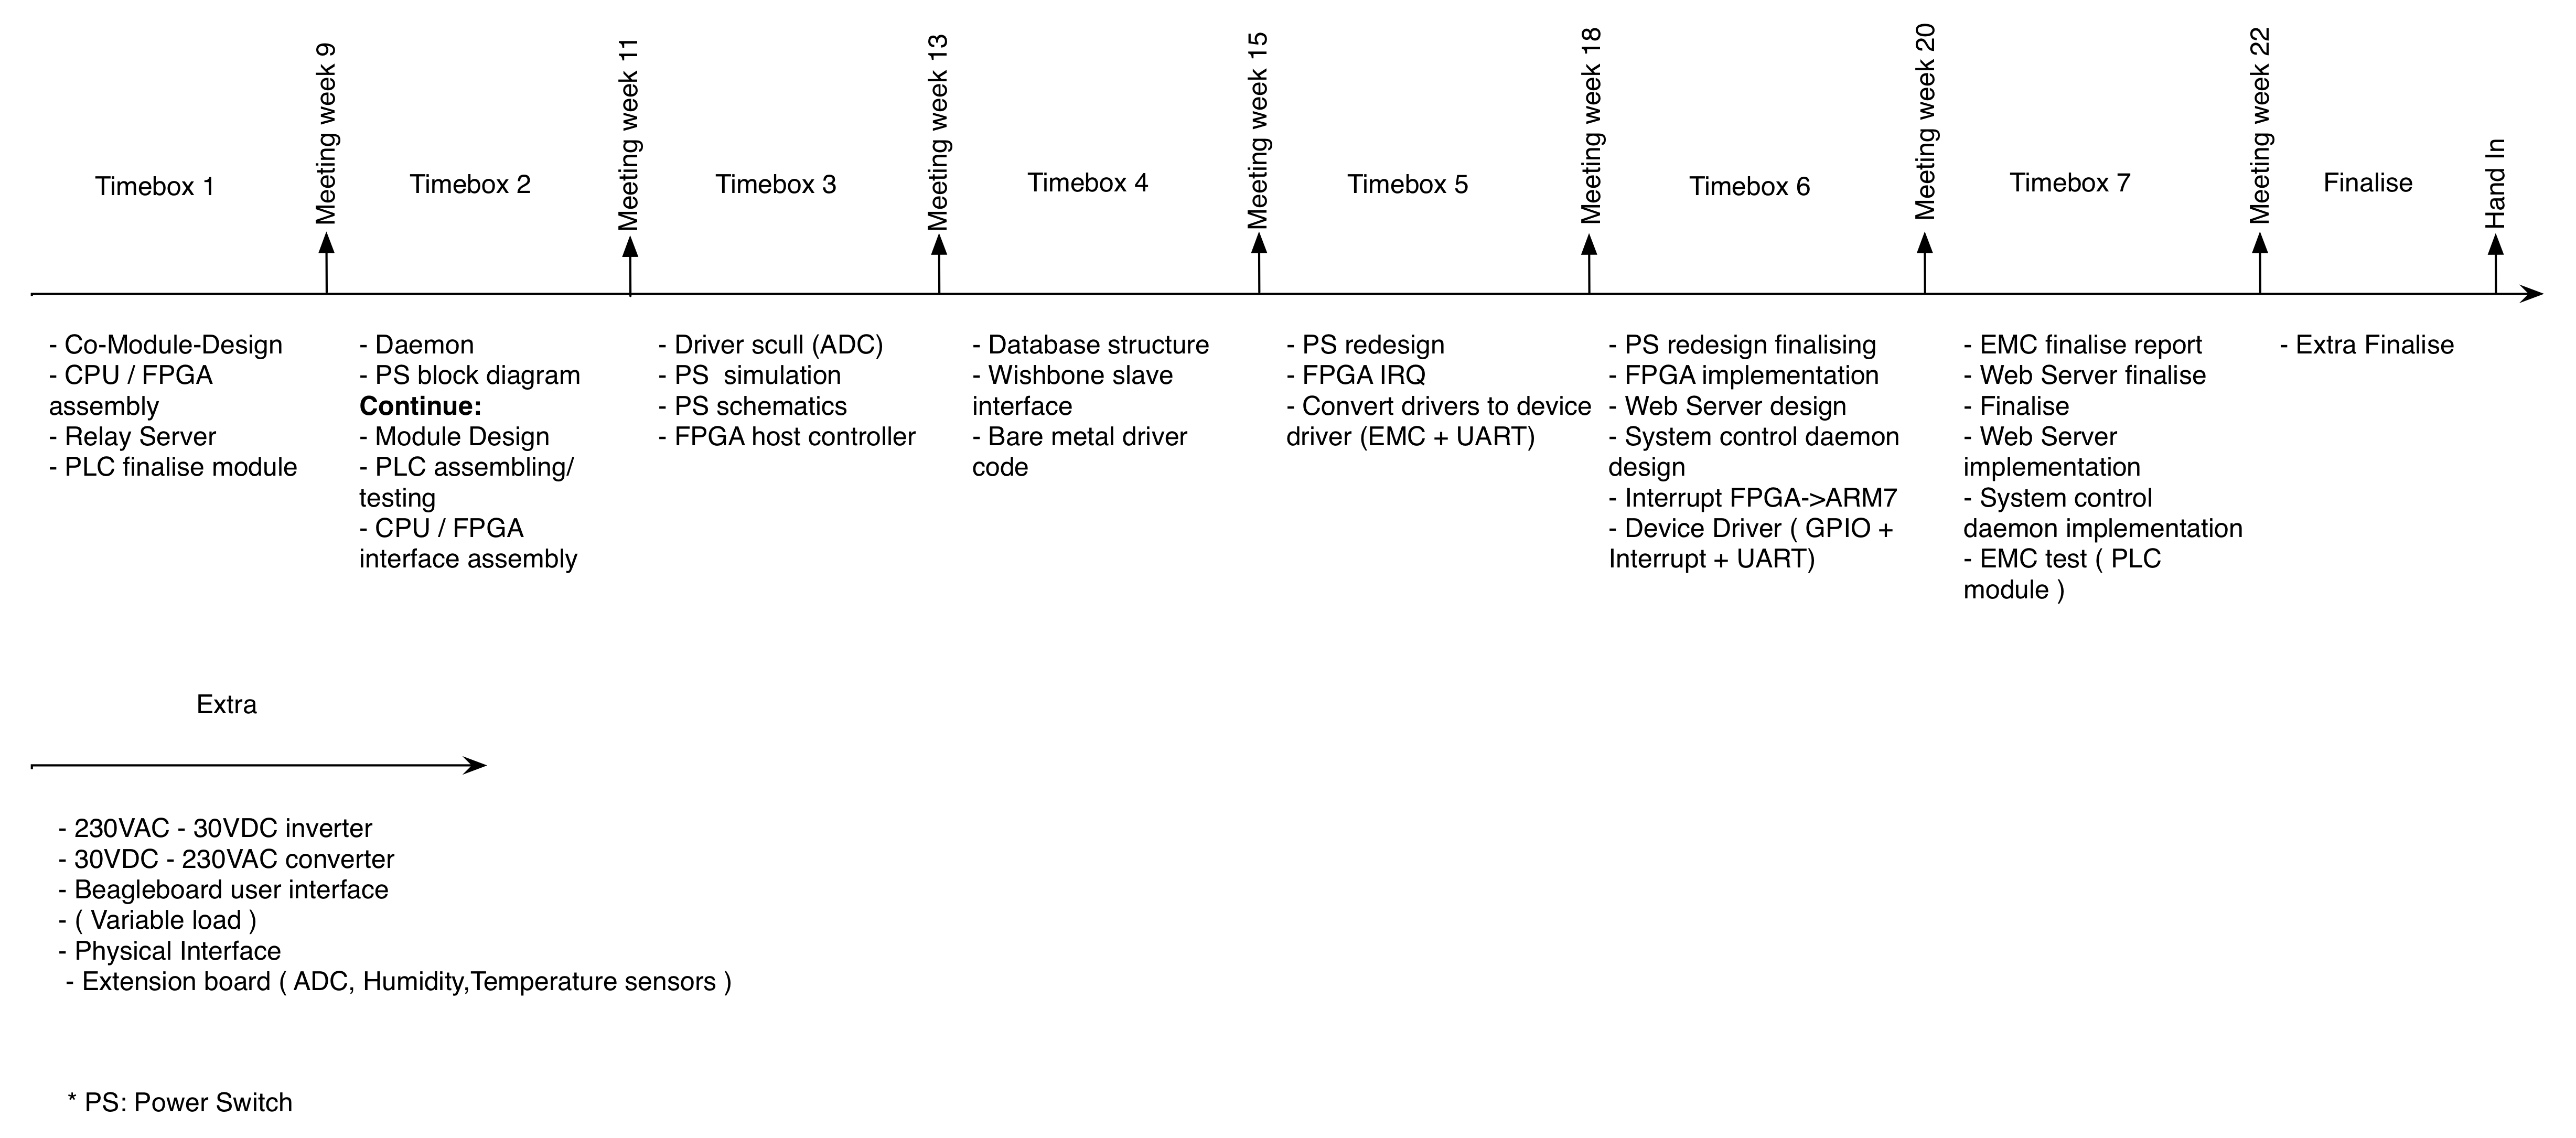
\includegraphics[width=1.0\textwidth]{images/tb_r5.png}
		%\caption{Updated time-box}
	\end{centering}
\end{figure}

\subsubsection{Work to be done in this time box}
\todo[inline]{Update List}
\begin{itemize}
	\item Switch interrupt
	\begin{itemize}
		\item debouncer
		\item Interrupt
	\end{itemize}
	\item Jesus thing
		\begin{itemize}
			\item sub thing
		\end{itemize}
	\item Dennis thing
	\begin{itemize}
		\item Sub thing
	\end{itemize}
\end{itemize}

\paragraph{Description:}
\todo[inline]{Update Description}
\begin{description}
	\item[Switch interrupt] In order to send data to the interrupt register, an interrupt output for the switch block has to be implemented, and the switches has to be debounced, to secure that the interrupt data is send only once.
	\item[Jesus thing]
	\item[Dennis thing]
\end{description}

\subsubsection{Time planning}

\begin{table}[H]
\centering
	\todo[inline]{Update Time}
	\begin{tabular}{|l|c|c|c|c|c|}
		\hline
		~			& Theis thing			& Jesus thing		& Dennis thing	\\ \hline
		Estimation	& 12					& xx				& xx			\\
		Actual		& 20					& xx				& xx			\\
		Developer	& Theis					& Paulo				& Dennis		\\
		\hline
	\end{tabular}
	\caption{Estimation and actual time used on the project}
\end{table}
% % % % % % % % % % % % % % % % % % % % % % % % % % % % % % % % % % % % % % % % %
% % % % % % % % % % % % % % % % % % % % % % % % % % % % % % % % % % % % % % % % %
% Theis Thing
% % % % % % % % % % % % % % % % % % % % % % % % % % % % % % % % % % % % % % % % %
\subsection{Switch interrupt - Theis}
%			Intro
%					verification specification
%					deployment specification
%
This part is, together with the interrupt register from earlier timebox a way to tune performance in reading and writing between the Spartan 6 and the LPC2478.
\subsubsection{Analysis}
%			Analysis
%
%                Refactored block diagram
%                Refactored class diagram
%                Detailed use cases
%                User interface specification
%                System interface specification
%                Dimensioning specification 
%
The interrupt block in the Spartan 6 is the switch block. The switch block needs to be redesign in order to get an interrupt output to the interrupt register, the switches also needs to be debounced, to prevent it from sending the same interrupt data more than once. Two output is added to the switch block, one single bit for interrupt indication and a 7 bit vector for the data to the interrupt register. Inside the block a finite state machine is made for denouncing the switches. Below the redesigned switch block is shown.

\begin{figure}[H]
	\begin{centering}
		%\missingfigure{Updated timebox figure}
		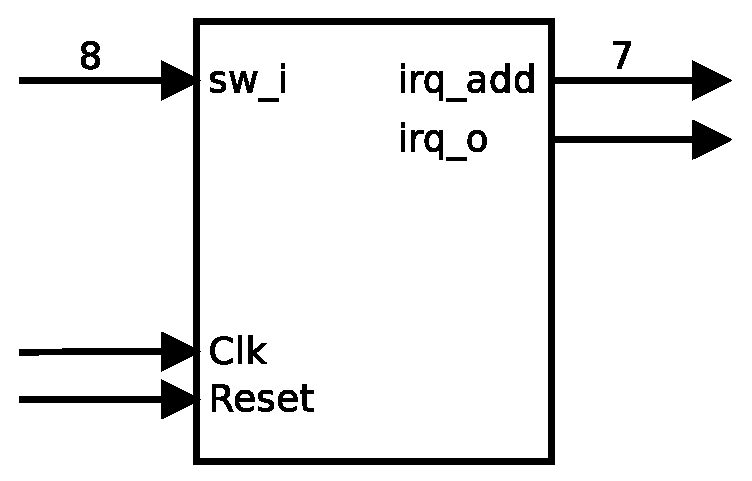
\includegraphics[width=0.3\textwidth]{images/tb6_switchblock.eps}
		\caption{Updated switch block}
	\end{centering}
\end{figure}


\subsubsection{Design}
%       	 Design
%
%                UML/SysML deployment view(s)
%                Mechanical specifications and dimensioning
%                HW module specification per block
%                UML SW deployment view
%                Class specification
%                Refactored class diagram
%                Use case scenarios specifications
%                Sequence diagrams
%
Because of switch bounce, the block needs to take care of this. Below a picture of switch bouncing is shown. The problem is every time the signal goes high the switch block will send data to the interrupt register, to prevent this the block compare a delayed input signal to the present signal, and first when the signal is stable, the system will react on the input.

\begin{figure}[H]
	\begin{centering}
		%\missingfigure{Updated timebox figure}
		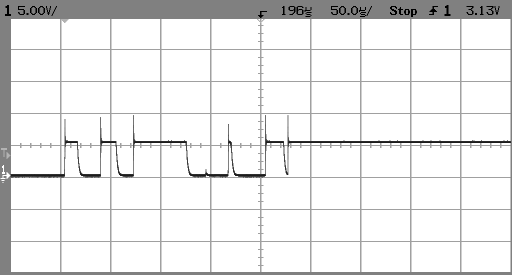
\includegraphics[width=0.5\textwidth]{images/tb6_bounce.png}
		\caption{Switch bouncing}
	\end{centering}
\end{figure}

To debounce the switch a state machine for the switch block is made. This diagram is shown below. The start box set the start output signal to the input signal. The interrupt signal is set high in the OUT0 state, and low again in the IDLE state after the "q2" delay. This is done to have the interrupt signal high enough time for the interrupt register to save the data. The "q1" delay is used to compare the input signal with the output signal in order to capture changes on the 8 switches.

\begin{figure}[H]
	\begin{centering}
		%\missingfigure{Updated timebox figure}
		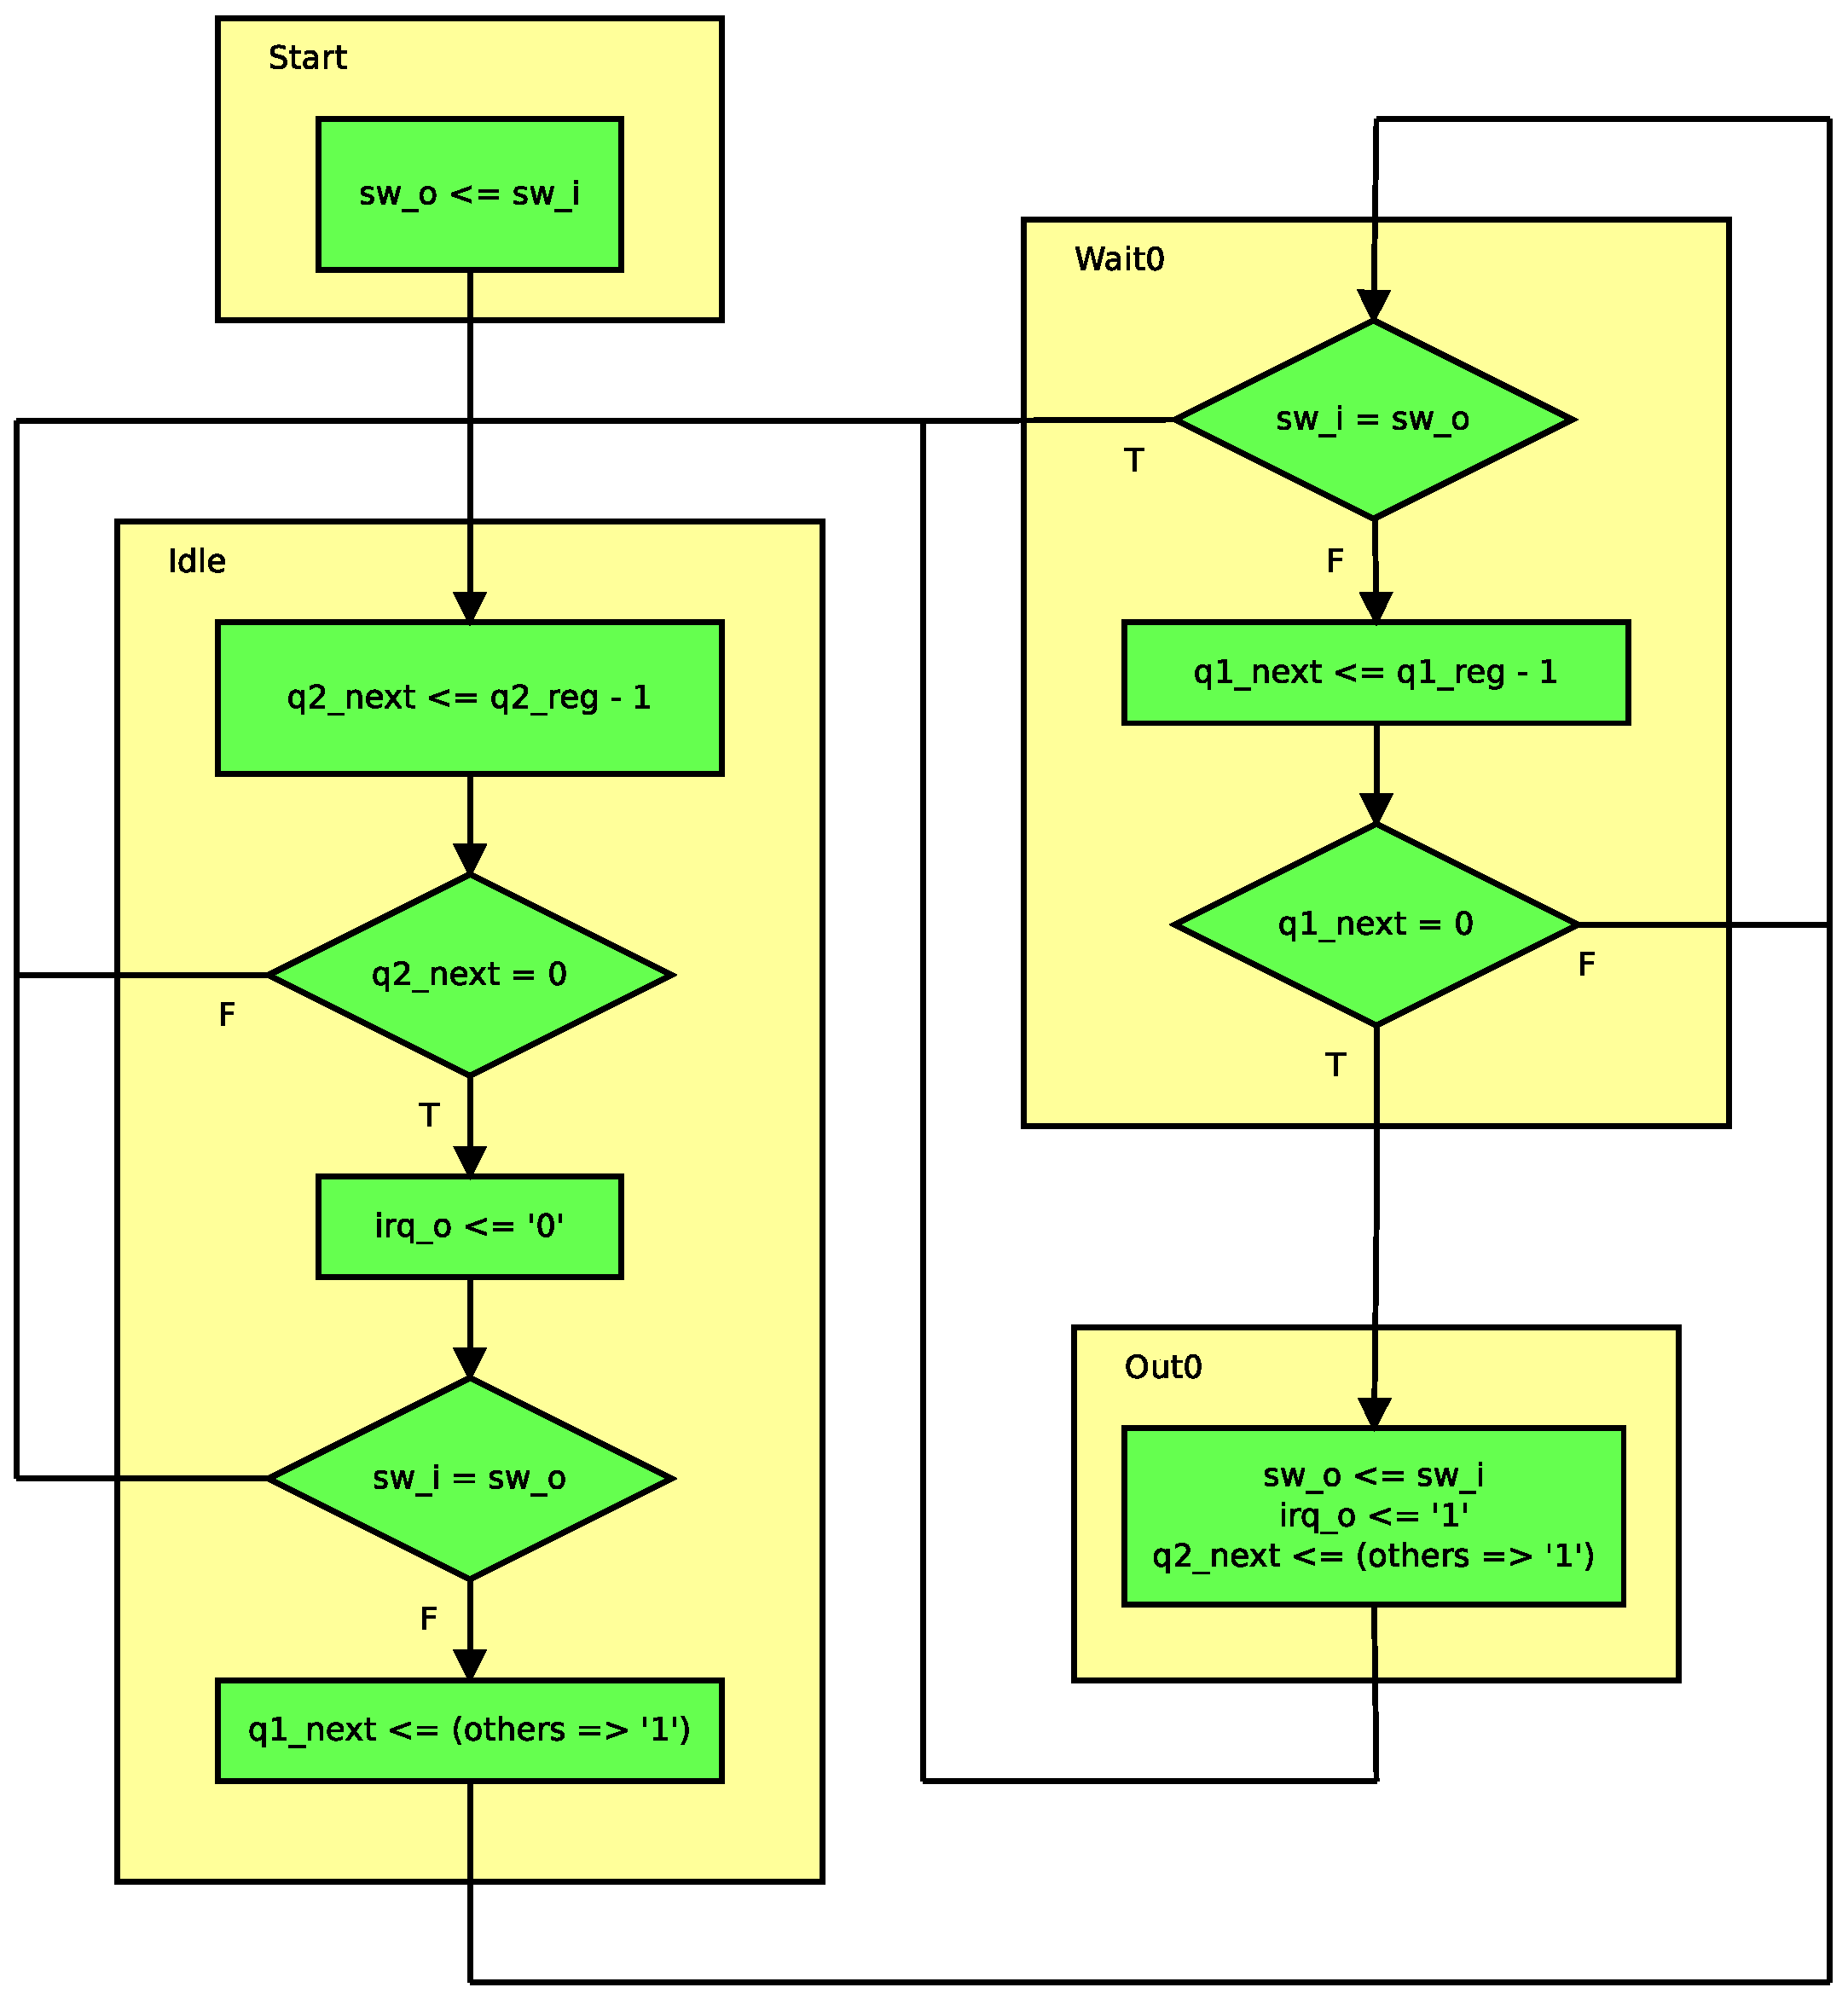
\includegraphics[width=0.7\textwidth]{images/tb6_switch_FSD.eps}
		\caption{Switch block state machine}
	\end{centering}
\end{figure}

\subsubsection{Implementation}
%     	   Implementation
%
%                Mechanical drawings with details explained
%                Electronic diagrams with details explained
%                Source code with details explained
%                Description of integration 
%
The code for the IDLE state is shown below, here the "q2" delay is used in the start, then the interrupt pin is set to zero, then the input and output is compared, if they are not equal the next state is WAIT0 and the "q1" delay is set.
\begin{lstlisting}[language=VHDL]
...
when IDLE =>
	q2_next <= q2_reg-1;
	if	(q2_next = 0) then
		irq_o <= '0';
		if	(sw_i = sw_o) then
			state_next <= IDLE;
		else
			q1_next		<= (others => '1');
			state_next	<= WAIT0;
		end if;
	else
		state_next <= IDLE;
	end if;
...
\end{lstlisting}
In the WAIT0 state the input and output is compared repeatedly to check if the input is stable. If the input is stable long enough time the OUT0 state is entered.
\begin{lstlisting}[language=VHDL]
...
when WAIT0 =>
	if	(sw_i = sw_o) then
		state_next <= IDLE;
	else
		q1_next <= q1_reg-1;
		if	(q1_next = 0) then
			state_next <= OUT0;
		else
			state_next <= WAIT0;
		end if;
	end if;
...
\end{lstlisting}
In the OUT0 state the switch output is set to switch input signal, and an interrupt signal is set high, the "q2" delay is set and it returns to the IDLE state.
\begin{lstlisting}[language=VHDL]
...
when OUT0 =>
	sw_o		<= sw_i;
	irq_o		<= '1';
	q2_next		<= (others => '1');
	state_next	<= IDLE;
...
\end{lstlisting}

\subsubsection{Verification}
%       	 Verification
%
%                Module tests
%                Integration tests
%                Acceptance test
The code is tested on a test bench in isim. The test verify that the block first set the switch output after the input has been stable for a while. And when the output is set the interrupt signal is set high for some time and then set low again. 
\begin{figure}[H]
	\begin{centering}
		%\missingfigure{Updated timebox figure}
		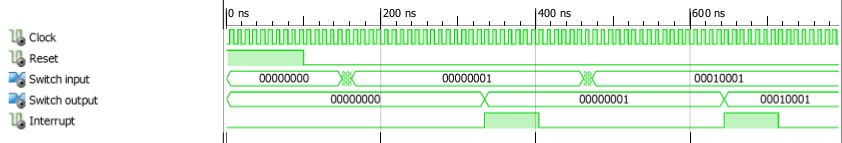
\includegraphics[width=1.0\textwidth]{images/tb6_switch_tb.png}
		\caption{Switch block test bench}
	\end{centering}
\end{figure}
\subsubsection{Conclusion}
% % % % % % % % % % % % % % % % % % % % % % % % % % % % % % % % % % % % % % % % %
% % % % % % % % % % % % % % % % % % % % % % % % % % % % % % % % % % % % % % % % %
% Jesus Thing
% % % % % % % % % % % % % % % % % % % % % % % % % % % % % % % % % % % % % % % % %
\subsection{WebServer - Paulo}
%			Intro
%					verification specification
%					deployment specification
%
In time box 4 a web server was implemented at the ip address 10.1.18.223, this is a virtual machine assign as development environment for the uClinux distribution. The server is running Apache 2, PHP version 5.1.6 and MySQL server 5.0.95.
In this time box a web services system is developed for the communication between the Embedded device and the web server and the other way around. The web page made in Project 3 is incorporated with server side scripts for a fully functional web interface.
\subsubsection{Analysis}
%			Analysis
%
%                Refactored block diagram
%                Refactored class diagram
%                Detailed use cases
%                User interface specification
%                System interface specification
%                Dimensioning specification 
%
For a fully functional web interface the communication have to present in both direction since some teams need to send commands from them web page to the modules.
For the fully cooperation with all the teams a file structure was created in the server, where each team have is own folder where all the needed scripts, images and layout styles can be implemented without changing the main layout approved in project 3.
\lineparagraph{Web interface file Structure}
\begin{itemize}
	\item index.php
	\item savedata.php
	\item sendcmd.php
	\item saveip.php
	\item ajax.js
	\item login.php 
	\item cron.php 
	\item includes\/ 
	\begin{itemize}
		\item db\_connect.php
		\item db\_globals.php
	\end{itemize} 
	\item modules\/ 
		\begin{itemize}
		\item photovoltaic\/ 
			\begin{itemize}
				\item index.php
				\item db\_connect.php
				\item cron.php 
				\item (Each team choose the rest of the scripts) 
			\end{itemize}
		\item caes\/ 
			\begin{itemize}
				\item index.php 
				\item db\_connect.php 
				\item cron.php 
				\item (Each team choose the rest of the scripts) 
			\end{itemize}
		\item hub\/
			\begin{itemize} 
				\item index.php 
				\item db\_connect.php 
				\item cron.php 
				\item (Each team choose the rest of the scripts) 
			\end{itemize}
		\item battery\/ 
			\begin{itemize}
				\item index.php 
				\item db\_connect.php 
				\item cron.php 
				\item (Each team choose the rest of the scripts) 
			\end{itemize}
		\item windturbine\/ 
			\begin{itemize}
				\item index.php 
				\item db\_connect.php 
				\item cron.php 
				\item (Each team choose the rest of the scripts)
			\end{itemize}
	\end{itemize}
\end{itemize}

A short description for each script can be seen bellow:
\begin{itemize}
	\item index.php - First page of the web interface.
	\item savedata.php - Webservice that save data retrieved from the module to the database.
	\item sendcmd.php - Webservice to send commands to the desired module in the system.
	\item saveip.php - Webservice necessary to save the ip address of the energy hub, this will keep the system up and running even if a change on the network is made.
	\item ajax.js - This Javascript handle AJAX requests when the page have no need to be reloaded, that ensure less bandwidth in the web server.
	\item login.php  - This PHP script makes the authentication of the user, creating a session when the user gives the right certifications.
	\item cron.php  - Cron jobs are running by the server in a predefined time, in this case the cron.php at the web server root will point to the cron jobs inside each module folder.
	\item db\_connect.php - Handle the connection to the MySQL database.
	\item db\_globals.php - Includes all the global variables with the credentials for the database.
\end{itemize}

\lineparagraph{Communication}
The server have to be able to save the data retrieved from the system and send commands to the the modules connected to the energy hub. Web services are created for this functionalities.

Bellow we have the flow of the communication from the user until the final destination in this case the module or the energy hub.
\begin{figure}[H]
	\begin{centering}
		\missingfigure{Communication SendCmd.php}
		%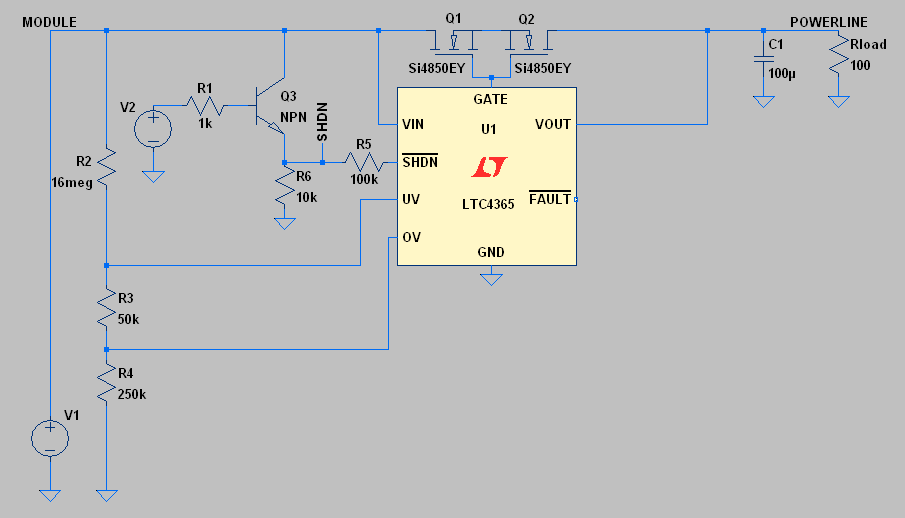
\includegraphics[width=1\textwidth]{images/tb5_LTC_simu1.png}
		%\caption{Schematics for the device LTC4365}
	\end{centering}
\end{figure}

This script doesn't give any feedback to the user, the commands send are not verified by the web server or the energy hub. The commands are handle by each module. With this system the flexibility of the system is ensured, since new modules can be added with different functionalities from the already known.
An application running in background at the energy hub uClinux, ensure that the command is translated to UART so it can be send through the power line communication to the modules.
\\\\
Measurements to be saved in the database:
\begin{figure}[H]
	\begin{centering}
		\missingfigure{Communication SendCmd.php}
		%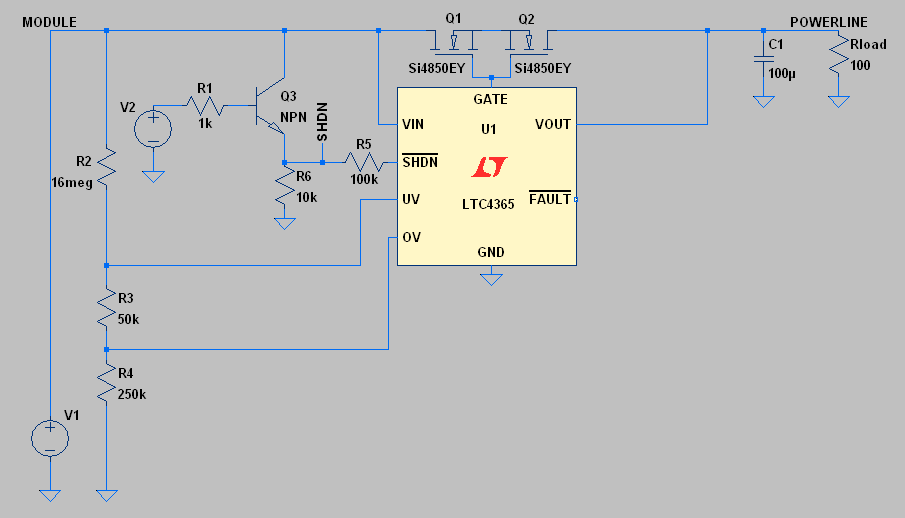
\includegraphics[width=1\textwidth]{images/tb5_LTC_simu1.png}
		%\caption{Schematics for the device LTC4365}
	\end{centering}
\end{figure}
To retrieve the measurements from the modules, an application running at the energy hub translate the data retrieved from the module through PLC to a URL request at the web server. In the server side the web server will collect the data and save it in the database.
\\\\
IP address is send from the Embedded Device:
\begin{figure}[H]
	\begin{centering}
		\missingfigure{Communication SendCmd.php}
		%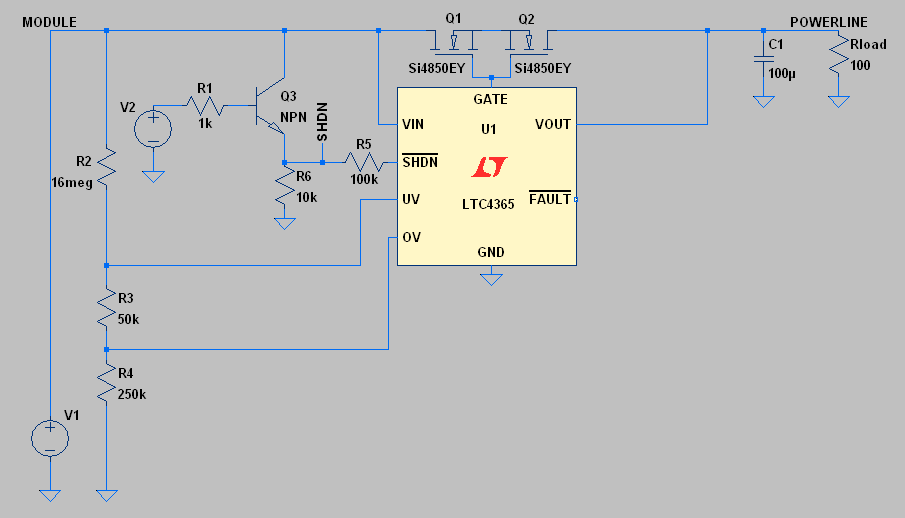
\includegraphics[width=1\textwidth]{images/tb5_LTC_simu1.png}
		%\caption{Schematics for the device LTC4365}
	\end{centering}
\end{figure}
A background application running at the uClinux, ensure that after reset the system IP address assigned by DHCP to the energy hub is saved in the database so commands can be send through the web interface. This add flexibility to the system, since a change in the network could stop the normal work of the system.

\subsubsection{Design}
%       	 Design
%
%                UML/SysML deployment view(s)
%                Mechanical specifications and dimensioning
%                HW module specification per block
%                UML SW deployment view
%                Class specification
%                Refactored class diagram
%                Use case scenarios specifications
%                Sequence diagrams
%
\subsubsection{Implementation}
%     	   Implementation
%
%                Mechanical drawings with details explained
%                Electronic diagrams with details explained
%                Source code with details explained
%                Description of integration 
%
\subsubsection{Verification}
%       	 Verification
%
%                Module tests
%                Integration tests
%                Acceptance test
\subsubsection{Conclusion}
% % % % % % % % % % % % % % % % % % % % % % % % % % % % % % % % % % % % % % % % %
% % % % % % % % % % % % % % % % % % % % % % % % % % % % % % % % % % % % % % % % %
% Dennis Thing
% % % % % % % % % % % % % % % % % % % % % % % % % % % % % % % % % % % % % % % % %
\subsection{Dennis thing - Dennis}
%			Intro
%					verification specification
%					deployment specification
%
\subsubsection{Analysis}
%			Analysis
%
%                Refactored block diagram
%                Refactored class diagram
%                Detailed use cases
%                User interface specification
%                System interface specification
%                Dimensioning specification 
%
\subsubsection{Design}
%       	 Design
%
%                UML/SysML deployment view(s)
%                Mechanical specifications and dimensioning
%                HW module specification per block
%                UML SW deployment view
%                Class specification
%                Refactored class diagram
%                Use case scenarios specifications
%                Sequence diagrams
%
\subsubsection{Implementation}
%     	   Implementation
%
%                Mechanical drawings with details explained
%                Electronic diagrams with details explained
%                Source code with details explained
%                Description of integration 
%
\subsubsection{Verification}
%       	 Verification
%
%                Module tests
%                Integration tests
%                Acceptance test
\subsubsection{Conclusion}
% % % % % % % % % % % % % % % % % % % % % % % % % % % % % % % % % % % % % % % % %
% % % % % % % % % % % % % % % % % % % % % % % % % % % % % % % % % % % % % % % % %
% Deployment
% % % % % % % % % % % % % % % % % % % % % % % % % % % % % % % % % % % % % % % % %
\subsection{Deployment}
	%which versions of the prototype the customer will get
	%with what functionality.
\paragraph{Theis thing}
%
%
\paragraph{Jesus thing}
%
%
\paragraph{Dennis thing}
%
%